\part{Historisk Utvikling}
\chapter{Bruddet med Klassisk Fysikk}
\section{Hva er Kvantemekanikk?} 
Kvantemekanikk forsøker å beskrive fysiske systemer på kvante nivå. Her står Schrödinger's likning sentralt. 

\subsection{Energikvantisering}
Energi i Kvantemekanikken er ikke en kontinuerlig størrelse. Den har diskrée verdier. Dette kalles energikvantisering. Dette gjelder både fotoner og elektroner. 

\subsection{Bølge-Partikkel-dualitet}
Vi vet ikke helt hva er partikkel er, men det vi vet er at de har egenskaper som minner om partikler og bølger. Dette kalles bølge-partikkel-dualiteten. Vi kan skyte ut fotoner i små energi pakker eller kvanter hvor de vil oppføre seg som partikler, men som en ser i dobbelspalteeksperimentet kan de likevel oppføre seg som bølger på samme tid. Da trenger vi Schrödinger's bølgeligning.

\subsection{Egentilstand og superposisjon}
En partikkel med kvantisert energien $ ϵ_{n} $ befinner seg i en tilstand som er beskrevet av bølgefunksjonen $ ψ_{n} $. Dette kalles en energi-egentilstand. En partikkel kan være i flere energi-egentilstander samtidig. Dette kalles superposisjon. Vi kan tenke på Schrödinger's katt som en partikkel som er i en superposisjon av to energi-egentilstander, død og levende. Da får vi følgende:
\begin{equation}
ψ = c_{\text{død}} ⋅ ψ_{\text{død}} + c_{\text{levende}} ⋅ ψ_{\text{levende}}
\end{equation}
Hvis vi måler tilstanden til katten vil vi få én av de to tilstandene. Enten død eller levende. Da ender vi opp i det som kalles \textit{egentilstand} fra bølgefunksjonen/superposisjon. Sannsynligheten for at katten er død er da $ \left\vert c_{\text{død}} \right\vert ^{2} $ og Sannsynligheten for at katten er levende er $ \left\vert c_{\text{levende}} \right\vert ^{2} $. Det eneste Kvantemekanikken kan fortelle oss er sannsynligheten for at katten er i en tilstand, ikke om den er i den tilstanden eller ikke, før vi måler det. 

\subsection{Heisenberg's uskarphetsrelasjon}
I klassisk mekanikk er foreksempel posisjon $ \mathbf{x} $ og bevegelsesmengde $ \mathbf{p} $ uavhengig størrelser. I Kvantemekanikken impliserer via Heisenberg's uskarphetsrelasjon at en ikke kan observerer begge til en vilkårlig presisjon. Dette uttrykkes via følgende formel
\begin{equation}
Δ \mathbf{p} Δ\mathbf{x} \geq \frac{ℏ}{2}
\end{equation}
hvor $ Δ\mathbf{x} $ er usikkerheten i posisjon og $ Δ\mathbf{p} 
$ er usikkerheten i bevegelsesmengde. Dette er bare en merkbart på atomært nivå, men gjelder teknisk sett alltid. 

\subsection{Paulis eksklusjonsprinsipp}
To fermioner (f.eks elektroner, protoner, kvarker og nøytrinoer) akn ikke befinne seg i samme tilstand (dvs. samme energi samme sted). Dette ser vi i atomer hvor elektronene fyller opp skall slik at nye elektroner må fylle opp et nytt skall. 



\section{Enheter i Kvantefysikk}
\subsection{Lengde}
For å unngå ekstremt små eller store tall bruker vi litt smarte enheter. Kvantefysikken operer på størrelser fra $ 10^{-8} $ til $ 10^{18} $m. Nanometer (nm) er $ 10^{-9} $m, femtometer (fm) er $ 10^{-15} $m og ångstrøm (Å) er $ 10^{-10} $m / $ 0.1 $nm.

\subsection{Energi}
For energi brukes til vanlig Joule, men energien i kvantemekanikken er så liten som $ 10^{-19} $J. Da bruker vi eV (elektronvolt) som er $ 1.602 \cdot 10^{-19} $C. Dette kommer fra at 1J er likt med 1C $\cdot$ 1V. Da er 1 eV den kinetiske energien et elektron får når den akselereres gjennom en potensialdifferensen på 1V. 

\subsection{Masse}

Istedet for å bruke kg for å måle masse kan vi heller bruke MeV/c$^{2}$. Dette kommer fra likningen $ E = mc^{2} $. Ser vi på hvileenergien til med enheten eV får vi 
\begin{equation}
E_{0}^{\text{elektron}} = m_{e} c^{2} = 5.11 \cdot 10^{5} \text{eV}
\end{equation}
Løser vi dette for massen $ m_{e} $ får vi
\begin{equation}
m_e = E_{0}^{\text{elektron}} / c^{2} = 0.511\ \text{MeV}/c^{2}
\end{equation}

\subsection{Andre Konstanter}
\textbf{Placks konstant}
\begin{equation}
h = 6.626 ⋅  10^{-34} \text{ Js} = 4.135 ⋅ 10^{-15} \text{  eVs}
\end{equation}
\begin{equation}
ℏ = \frac{h}{2 \pi} = 1.055 ⋅ 10^{-34} \text{Js} = 6.582 ⋅ 10^{-16} \text{eVs} 
\end{equation}
\begin{equation}
hc = 1240 \text{ eV nm} (\text{MeV fm})
\end{equation}
\begin{equation}
ℏc = 197.3 \text{ eV nm} (\text{MeV fm})
\end{equation}
Noen ganger kan det lønne seg å gange en brøk med $ c $ oppe og nede for å få inn konstanten $ ℏc $. Utrykket under hadde medført veldig små størrelser ($ 10^{-34} $ og $ 10^{-31} $) og dermed ville det blitt vanskelig å regne med. 
\begin{equation}
\frac{h}{m_e c} = \frac{hc}{m_e c^{2}} = \frac{1240 \text{eV nm}}{0.511 ⋅ 10^{6}} ≈ 0.002 nm
\end{equation}
\subsection{Coulomb-potensialet}
\begin{equation}
V(r) = \frac{e^{2}}{4 \pi \epsilon_{0} r} = \frac{k_e e^{2}}{2}, \qquad k_e e^{2} = 1.44 \text{eV nm}
\end{equation}
\subsection{Nyttige Tabeller}

\begin{figure}[ht!]
  \centering
  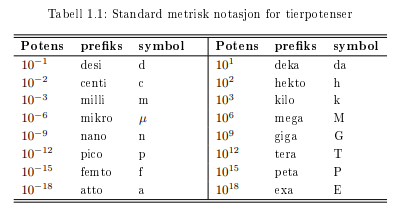
\includegraphics[scale = 1]{Figures/Metric power notation.png}
  \caption{}
  \label{fig: Metric power notation}
\end{figure}

\begin{figure}[ht!]
  \centering
  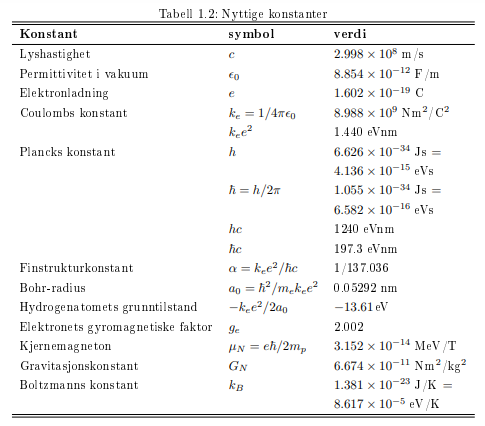
\includegraphics[scale = 1]{Figures/Constants table.png}
  \caption{}
  \label{fig: Constants table}
\end{figure}

\begin{figure}[ht!]
  \centering
  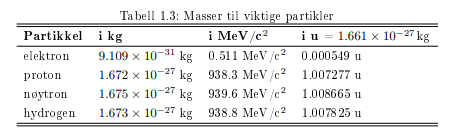
\includegraphics[scale = 1]{Figures/Masser til viktige partikler.png}
  \caption{}
  \label{fig: Masser til viktige partikler}
\end{figure}

\begin{figure}[ht!]
  \centering
  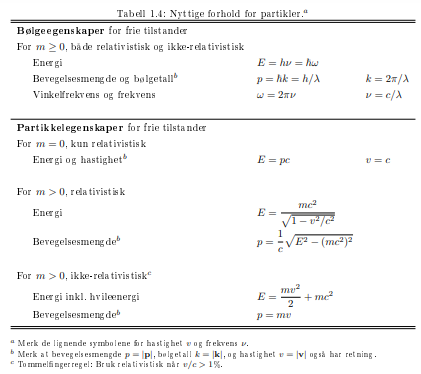
\includegraphics[scale = 1]{Figures/Nyttige forhold for partikler.png}
  \caption{}
  \label{fig: Nyttige forhold for partikler}
\end{figure}

\newpage

\section{Planck's Kvantiseringshypotese}
Kvantisering betyr i kvantefysikken at en fysisk størrelse bare antar diskrete verdier. Eksempler på dette er elektrisk ladning, hvor fri ladning er et heltallig $ \mathbb{N} $ multiplum av antall frie elektroner. Energi kan også kvantifiseres og var definerende for bruddet med klassisk fysikk. Klassisk fysikk klarer ikke å forklare frekvensfordelingen til elektromagnetisk stråling fra et legeme ved en gitt temperatur. Dette kan være sola eller en vanlig stekeplate. 
\subsubsection*{Definisjoner}
\begin{itemize}
    \item \textbf{Termisk stråling}: Elektromagnetisk stråling sendt ut av et materiale ved en temperatur $T$. Alle legemer emitterer og absorber denne strålingen
    \item Ved en gitt temperatur $T$ er vi interessert i å finne fordelingen av emittert stråling som funksjon av den elektromagnetiske strålingen sin frekvens $ν$ eller bølgelengde $λ$. Forholdet mellom frekvens $ν$ og bølgelengde $λ$ er gitt ved
    \begin{equation}
    ν = \frac{c}{λ}
    \end{equation}
    
    \item \textbf{Frekvensfordeling}
    \begin{equation}
    M_{ν}(T)
    \end{equation}
    Kalles spektralfordelingen eller fordelingsfunksjonen for frekvensspekteret beskriver mengden utstrålt energi fra en gjenstand ved temperatur $ T $ per areal per tid per frekvensenhet. 
    
    \item Integrert over alle frekvenser 
    \begin{equation}
    M(T) = \int_{0}^{\infty} M_{ν}(T) \ dν
    \end{equation}
    får vi totalt utstrålt energi per sekund per areal ved en gitt temperatur $ T $. Enhetene bli følgende: M(T) = $ J / m^{2}s = W / m^{2} $. Dette kalles radians. 
    
    \begin{figure}[h!]
        \centering
        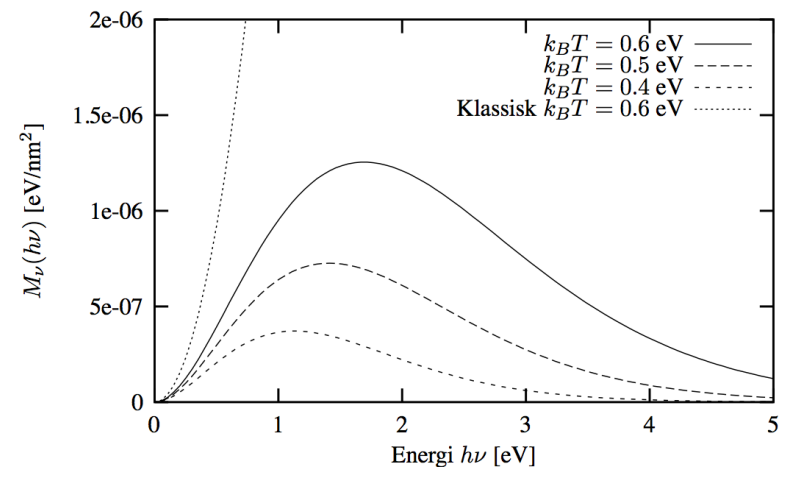
\includegraphics[scale = .5]{Figures/Frekvensfordeling kvantiserinspostulat.png}
        \caption{Frekvensfordelingen fra Planck's kvantiseringspostulat. Merk den klassiske kurven som øker alt for mye ikke matcher observert frekvens}
        \label{fig: Frekvensfordeling kvantiserinspostulat}
    \end{figure}
    
    \item \textbf{Vår utfordring er å finne frem til en forklaring for den eksperimentell formen til} $M_{ν}(T)$
\end{itemize}

Den klassiske versjonen å se på dette var via et sort legeme som er tenkt til å ikke reflektere noe av strålingen den mottar, alt blir absorbert. Dette ble det eksperimentert og resultatet ser man i figur \ref{fig: Frekvensfordeling kvantiserinspostulat}. 
Basert på måledata kom en fram til at radiansen til et sort legeme kan skrives som 
\begin{equation}
M(T) = σT^{4}
\end{equation}
hvor $σ$ er en konstant. Dette kalles Stefan-Boltzmanns lov. Wiens forskyvningslov beskriver sammenhengen mellom temperaturer og bølgelengden $λ_{\text{max}}$. 
\begin{equation}
λ_{\text{max}}T = 2.897 ⋅ 10^{-3} \text{ mK}
\end{equation}
Nå skal vi se hva som skjer når vi bruker resultatene fra klassisk fysikk. 
\begin{equation}
M_{ν}(T) = \frac{2 π ν^{2}}{c^{2}} \left< E \right>
\end{equation}
hvor $\left< E \right>$ er gjennomsnitsenergien per svingemode til det elektromagnetiske feltet i hulrommet til det sorte legeme. 
\begin{equation}
\left< E \right> = k_{B}T
\end{equation}
hvor $k_{B}$ er Boltzmanns konstant. For å finne radiansen setter vi inn utrykket for $\left< E \right>$ og integrerer. 
\begin{equation}
M(T) = \int_{0}^{∞} \frac{2 π v^{2}}{c^{2}} k_{B}T \ \mathrm{d}ν
\end{equation}
Dette er lett å se at energien går mot uendelig og matcher ikke med de eksperimentelle resultatene. En formel som matcher bedre kan ikke divergere. Feilen er at $\left< E \right>$ er ikke stemmer. Hvis en ser på strålingen som et stort antall kvantiserte enheter med energi $ϵ_{n}$
\begin{equation}
ϵ_{n} = nhν
\end{equation}
der $h$ er Planck's konstant og $n$ er et heltall. Planck utledet et alternativt utrykk for $\left< E \right>$. 
\begin{equation}
\left< E \right> = \frac{hν}{e^{hν/k_{B}T} - 1}
\end{equation}
Som gir
\begin{equation}
M_{ν}(T) = \frac{2 π ν^{2}}{c^{2}} \frac{hν}{e^{hν/k_{B}T} - 1}
\end{equation}
Som samsvarer med eksperiment. Viktig å få med seg er at $\left< E \right> → k_{B}T$ når $T → ∞$ eller $λ → \infty$ aka $ν → 0$ som er hvor klassisk mekanikk er gyldig.
For å få litt mer elegante utrykk å unngå store eller små tall ganger vi inn $h$. 
\begin{equation}
M_{ν}(T) = \frac{2π}{h^{2}c^{2}} \frac{(hν)^{3}}{e^{h ν/k_{B}T} - 1}
\end{equation}

Vi setter in $x = hν$
\begin{equation}
M_{x}(T) = \frac{2π}{h^{2}c^{2}} \frac{x^{3}}{e^{x/k_{B}T} - 1}
\end{equation}
Vi vet at $hc = 1240 $eV nm 
\begin{equation}
M_{x}(T) = \frac{2π}{1240^{2}} \frac{x^{3}}{e^{x/k_{B}T} - 1}
\end{equation}

Hvor $M_{x}$ har enheter eV / nm$^{2}$. For å utlede Stefan-Boltzmanns lov via Planck's utrykk bruker vi den originale formelen og setter in x vi fant tidligere. 
\begin{equation}
M(T) = \int_{0}^{∞} M_{ν}(T) \ \mathrm{d}ν = \int_{0}^{∞} \frac{2πν^{2}}{c^{2}} \frac{hν}{e^{hν / k_{B}T} - 1} \ \mathrm{d}ν
\end{equation} 

\begin{equation}
M(T) = \frac{2πk^{4}_{B}}{c^{2}h^{3}}T^{4} \underbrace{\int_{0}^{∞} \frac{x^{3}}{e^{x} - 1} \ \mathrm{d}x}_{\frac{π^{4}}{15}}
\end{equation}

\begin{equation}
M(T) = σT^{4}, \quad σ = \frac{2π^{5}k^{4}_{B}}{15c^{2}h^{3}} = 5.676 ⋅ 10^{-8} \frac{\text{W}}{\text{m}^{2} \text{K}^{4}}
\end{equation}

Den viktigste forskjellen var at Planck regnet ut den midlere verdien $\left< E \right>$ med diskrete verdier for energi og ikke kontinuerlige verdier. Han hadde dataen foran seg og prøvde å finne en modell som passet. 

\subsubsection*{Plank's Hypotese}
Enhver fysisk størrelse som utviser enkle harmoniske svingninger har energier som tilfredsstille
\begin{equation}
E_n(ν) = nhν, \qquad n = 1, 2, 3, \dots
\end{equation}

hvor $ν$ er frekvensen til svingningene og $h$ er en universell konstant. 

Kvantefysikken gjelder alltid, men klassisk fysikk kan brukes når energiskalaen er stor nok ettersom det ikke er merkbart. 

\subsection{Utledning av Wiens Forskyvningslov}